The field, force, and torque solutions outlined in Section \ref{sec:p1methodology} have been verified using both previous literature and finite element simulations. Firstly, the configuration used by \textcite{Akoun1984}\footnote{\textcite{Akoun1984} used two cuboidal magnets, each of dimensions 20mm by 12mm by 6mm with a vertical gap of 2mm between them.} was considered (Figure \ref{fig:p1akounyonnet}). Here, the force on magnet B is measured as it moves a distance \(d\) in the \(x\)-direction while magnet A remains fixed. Both magnets have parallel magnetisation vectors in the \(z\)-direction with a value of 0.38 Tesla. The resulting force and torque depends not only on magnetisation, but also on the geometry of the magnets.
\begin{figure*}
	\centering
	\begin{subfigure}{0.4\textwidth}
		\centering
		\tdplotsetmaincoords{70}{130}
		\begin{tikzpicture}[scale=0.2,tdplot_main_coords]
		\coordinate(b1) at (10,-6,3);
		\coordinate(b2) at (10,6,3);
		\coordinate(b3) at (-10,6,3);
		\coordinate(b4) at (-10,-6,3);
		\coordinate(b5) at (10,-6,-3);
		\coordinate(b6) at (10,6,-3);
		\coordinate(b7) at (-10,6,-3);
		
		\draw (b1) -- (b2) -- (b3) -- (b4) -- cycle;
		\draw (b5) -- (b6) -- (b7);
		\draw (b1) -- (b5);
		\draw (b2) -- (b6);
		\draw (b3) -- (b7);
		
		\coordinate(t1) at (2,-14,11);
		\coordinate(t2) at (2,6,11);
		\coordinate(t3) at (-10,6,11);
		\coordinate(t4) at (-10,-14,11);
		\coordinate(t5) at (2,-14,5);
		\coordinate(t6) at (2,6,5);
		\coordinate(t7) at (-10,6,5);
		
		\draw[fill=white] (t1) -- (t2) -- (t6) -- (t5);
		\draw[fill=white] (t2) -- (t3) -- (t7) -- (t6);
		\draw (t5) -- (t1) -- (t4) -- (t3);
		
		\coordinate(midpt) at (2,-4,8);
		\coordinate(end) at (12,-4,8);
		
		\draw[->,dashed] (midpt) -- (end);
		
		\node(d) at (14.5,-3,8.5) {\textit{d}};
		\node(A) at (0,6,0) {\text{A}};
		\node(B) at (-4,6,8) {\text{B}};
		\end{tikzpicture}
		\caption{}
	\end{subfigure}
	~ \hspace{1cm}
	\begin{subfigure}{0.4\textwidth}
		\centering
		\tdplotsetmaincoords{90}{180}
		\begin{tikzpicture}[scale=0.2,tdplot_main_coords]
		\coordinate(b1) at (10,-6,3);
		\coordinate(b2) at (10,6,3);
		\coordinate(b3) at (-10,6,3);
		\coordinate(b4) at (-10,-6,3);
		\coordinate(b5) at (10,-6,-3);
		\coordinate(b6) at (10,6,-3);
		\coordinate(b7) at (-10,6,-3);
		
		\draw (b1) -- (b2) -- (b3) -- (b4) -- cycle;
		\draw (b5) -- (b6) -- (b7);
		\draw (b1) -- (b5);
		\draw (b2) -- (b6);
		\draw (b3) -- (b7);
		
		\coordinate(t1) at (2,-14,11);
		\coordinate(t2) at (2,6,11);
		\coordinate(t3) at (-10,6,11);
		\coordinate(t4) at (-10,-14,11);
		\coordinate(t5) at (2,-14,5);
		\coordinate(t6) at (2,6,5);
		\coordinate(t7) at (-10,6,5);
		
		\draw[fill=white] (t1) -- (t2) -- (t6) -- (t5);
		\draw[fill=white] (t2) -- (t3) -- (t7) -- (t6);
		\draw (t5) -- (t1) -- (t4) -- (t3);
		
		\coordinate(midpt) at (2,-4,8);
		\coordinate(end) at (6,-4,8);
		
		\draw[->,dashed] (midpt) -- (end);
		\node(d) at (7,-3,8) {\textit{d}};
		
		\draw[->,thick] (-4,0,6.5) -- (-4,0,9.5);
		\node (M1) at (-2.5,0,8) {\textbf{M}};
		\draw[->,thick] (0,0,-1.5) -- (0,0,1.5);
		\node (M2) at (1.5,0,0) {\textbf{M}};
		
		\node (A) at (-8,6,0) {\text{A}};
		\node(B) at (-8,6,8) {\text{B}};
		
		\draw [->] (-15,-4,-3) -- (-12,-4,-3);
		\draw [->] (-15,-4,-3) -- (-15,-4,0);
		\node (x) at (-11,-4,-3) {\(x\)};
		\node (z) at (-15,-4,1) {\(z\)};
		\end{tikzpicture}
		\caption{}
	\end{subfigure}
	\caption{The geometry used in Akoun and Yonnet's work in 1984 \cite{Akoun1984} with both magnets having parallel magnetisation in the \(z\)-direction. Magnet B moves a distance \(d\) along the top of magnet A.}
	\label{fig:p1akounyonnet}
\end{figure*}

Algorithms \ref{alg:p1alg1} and \ref{alg:p1alg2} were implemented in Matlab R2017b (MathWorks, Inc., Natick, MA, USA), with a basic meshing process using triangular elements. The mesh was created by repeatedly bisecting each triangle edge and joining the three bisection points, converting the triangle into four smaller triangles, until all triangles in the mesh had area less than a threshold value. Algorithms \ref{alg:p1alg1} and \ref{alg:p1alg2} were applied to Akoun and Yonnet's geometry \cite{Akoun1984} to calculate force and torque values for varying displacement. The finite element package Maxwell3D in ANSYS Electronics Desktop 2018.0 (ANSYS, Inc., Berkeley, CA, USA) was used with adaptive meshing to obtain finite element solutions for the force and torque in this configuration. Additionally, the force solutions presented by \textcite{Akoun1984} and torque solutions presented by \textcite{Janssen2010a} were calculated using Matlab code from Robertson \cite{Robertson2013,Robertson}, with the torque being evaluated about the centre of magnet B. These results were compared to those obtained with Algorithms \ref{alg:p1alg1} and \ref{alg:p1alg2} as well as finite element simulations.
\begin{figure*}
	\centering
	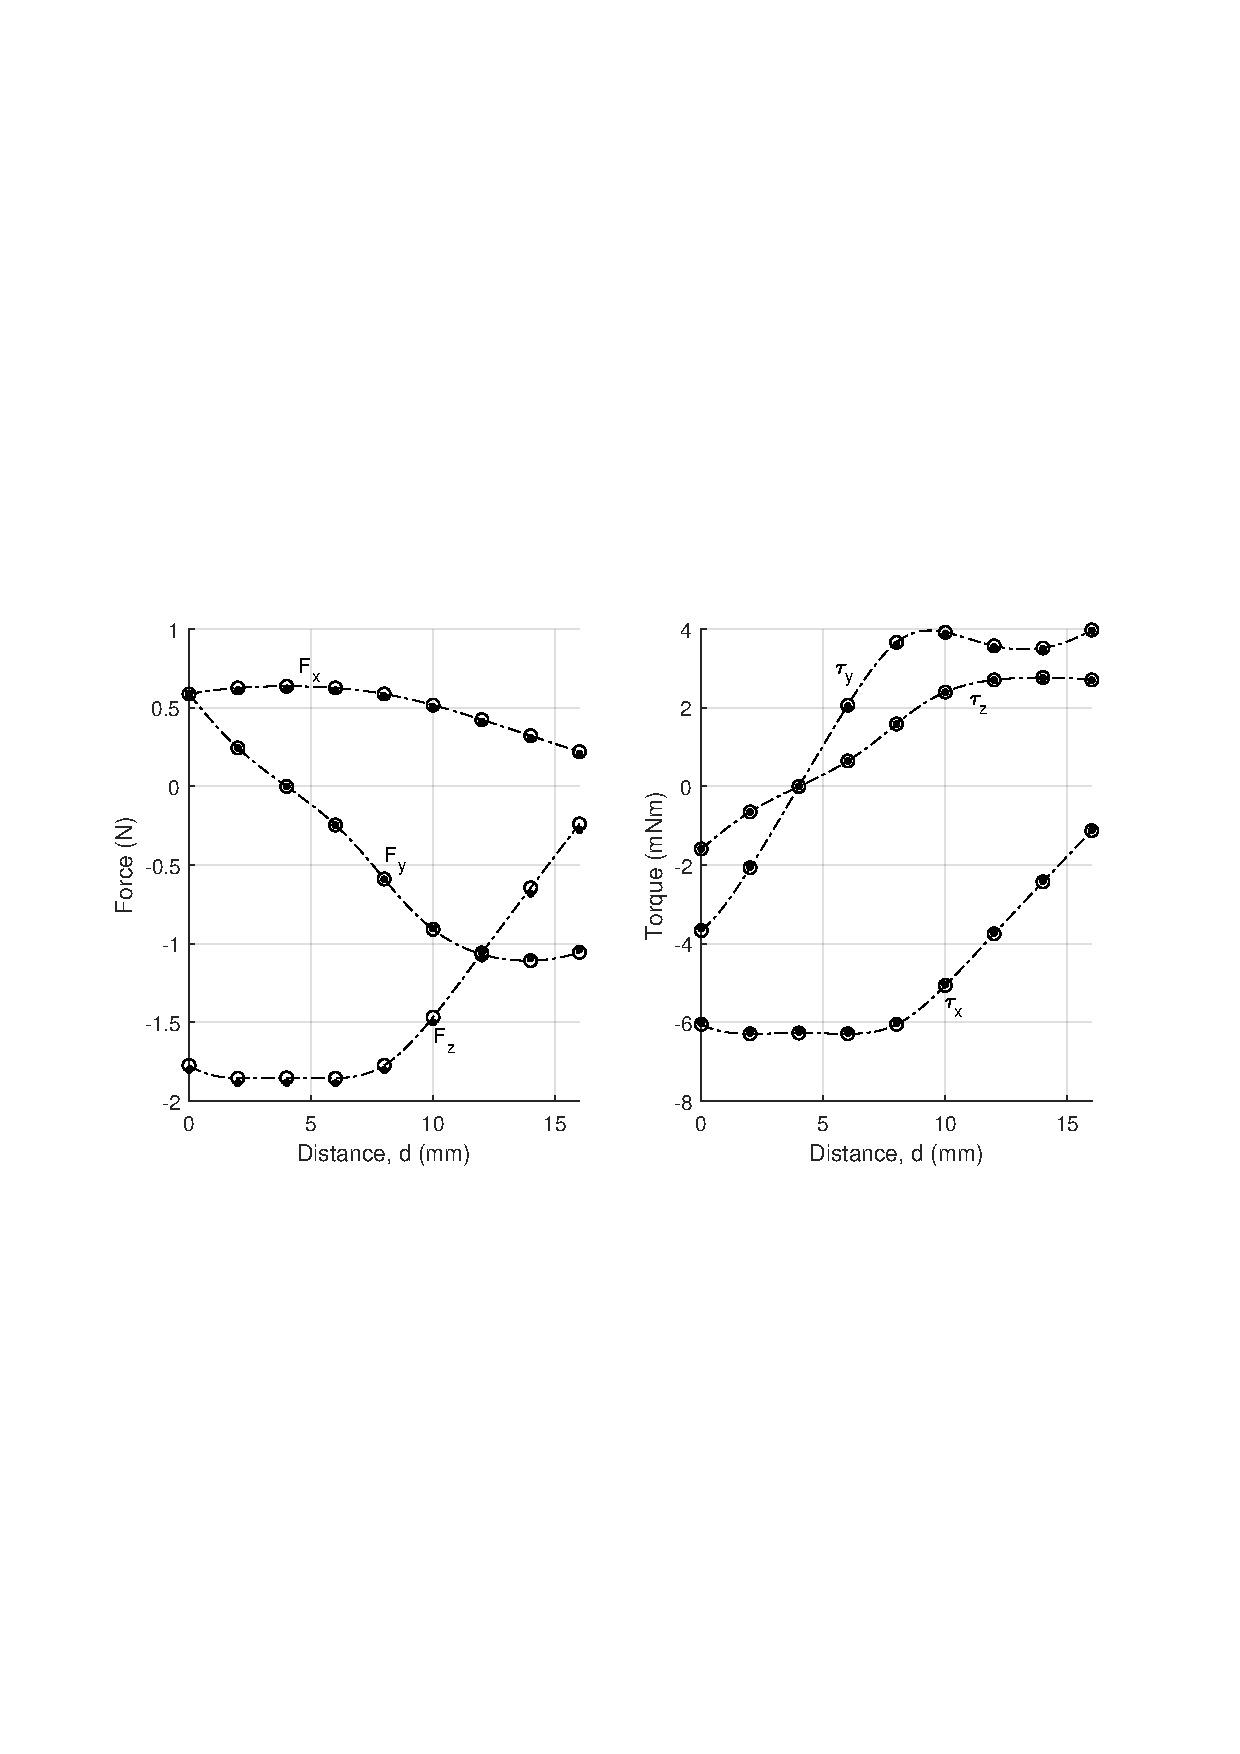
\includegraphics[trim = 3cm 9cm 3cm 9cm,width=0.9\linewidth]{p1/p1FIG4}
	\caption{Forces and torques on magnet B shown in Figure \ref{fig:p1akounyonnet} as it moves a distance \(d\) along the top of the magnet A. The dashed lines represent the results calculated from Algorithms \ref{alg:p1alg1} and \ref{alg:p1alg2}, with circles representing analytic solutions \cite{Akoun1984,Janssen2010a} and dots representing solutions obtained from a finite element simulation (Maxwell3D, ANSYS Electronics Desktop 2018.0). The values obtained with Algorithms \ref{alg:p1alg1} and \ref{alg:p1alg2} are in excellent agreement with the other two methods, especially the analytic solutions, indicating this work produces correct results for cuboidal magnets.}
	\label{fig:p1cuboidcase}
\end{figure*}

The three sets of results are shown in Figure \ref{fig:p1cuboidcase}. The forces and torques obtained from Algorithms \ref{alg:p1alg1} and \ref{alg:p1alg2} align with both the values from the finite element simulation and from the analytic solution, validating the algorithms for simple cuboidal magnets with parallel magnetisation. However, this test does not consider non-cuboidal magnets or non-parallel magnetisation and these must be considered for further validation.

Algorithms \ref{alg:p1alg1} and \ref{alg:p1alg2} were significantly faster than the finite element simulations when implemented in Matlab R2017b (MathWorks, Inc., Natick, MA, USA) on a workstation PC with an Intel Xeon E3-1240 v5 (3.50GHz) with 4 cores. Algorithms \ref{alg:p1alg1} and \ref{alg:p1alg2} completed each force calculation in approximately 0.65 seconds using 3072 triangular elements on the surface of magnet B, while the finite element simulations took a minimum of 30-40 seconds using an adaptive setup with a percent error of 1\% and approximately 17000 tetrahedral elements. Additionally, Algorithms \ref{alg:p1alg1} and \ref{alg:p1alg2} were considerably more accurate, achieving a maximum force error of 4.3 milliNewtons and a maximum torque error of 0.03 milliNewton-metres when compared to the analytic solutions, while the finite element solutions gave a maximum force error of 37 milliNewtons and a maximum torque error of 0.14 milliNewton-metres.

To validate Algorithms \ref{alg:p1alg1} and \ref{alg:p1alg2} for a more general case, two dodecahedral magnets were considered (Figure~\ref{fig:p1dodecahedra}). Both magnets are regular dodecahedra with edge lengths of 20mm and volumes of 61305mm\(^3\). Magnet B has magnetisation in the \(x\)-direction and may move vertically, while magnet A has magnetisation in the \(z\)-direction and is fixed. Both magnets have a unit magnetisation strength \(\mathbf{M}\), i.e. 1 Tesla. The \(x\)-force and \(y\)-torque on magnet B are calculated, with the torque calculated about its centre. The \(y\)- and \(z\)-forces, as well as the \(x\)- and \(z\)-torques are almost zero and thus neglected. The magnetic configuration was input into Algorithms \ref{alg:p1alg1} and \ref{alg:p1alg2} as well as a  three-dimensional finite element simulation, with the results shown in Figure \ref{fig:p1dodecahedraresults}\footnote{Due to the numeric nature of the force and torque calculations, accuracy is reduced when magnets are extremely close and an insufficient surface mesh density is used. As such, the magnets were limited to a minimum separation of 1mm.}. Due to symmetry, the forces in the \(y\) and \(z\) directions, as well as the torques about the \(x\) and \(z\) axes are extremely small and therefore not plotted in the figure.
\begin{figure*}
	\centering
	\begin{subfigure}{0.49\textwidth}
		\centering
		\tdplotsetmaincoords{70}{110}
		\begin{tikzpicture}[scale=50,tdplot_main_coords]
		\coordinate(p1t) at (0.026180,0.008506,0.005258);
		\coordinate(p2t) at (0.016181,-0.005257,-0.022270);
		\coordinate(p3t) at (0.009999,-0.013765,0.022270);
		\coordinate(p4t) at (0.000000,-0.027527,-0.005258);
		\coordinate(p5t) at (-0.000000,0.027527,0.005258);
		\coordinate(p6t) at (-0.009999,0.013765,-0.022270);
		\coordinate(p7t) at (-0.016181,0.005257,0.022270);
		\coordinate(p8t) at (-0.026180,-0.008506,-0.005258);
		\coordinate(p9t) at (0.016180,0.022271,-0.005256);
		\coordinate(p10t) at (0.010001,0.013765,-0.022270);
		\coordinate(p11t) at (-0.010001,-0.013765,0.022270);
		\coordinate(p12t) at (-0.016180,-0.022271,0.005256);
		\coordinate(p13t) at (0.016180,0.005257,0.022271);
		\coordinate(p14t) at (0.000001,-0.017012,-0.022271);
		\coordinate(p15t) at (-0.000001,0.017012,0.022271);
		\coordinate(p16t) at (-0.016180,-0.005257,-0.022271);
		\coordinate(p17t) at (0.026180,-0.008506,-0.005257);
		\coordinate(p18t) at (0.016180,-0.022271,0.005257);
		\coordinate(p19t) at (-0.016180,0.022271,-0.005257);
		\coordinate(p20t) at (-0.026180,0.008506,0.005257);
		
		\coordinate(p1b) at (0.016180,0.022270,-0.049242);
		\coordinate(p2b) at (0.016180,0.005258,-0.076770);
		\coordinate(p3b) at (0.016180,-0.005258,-0.032230);
		\coordinate(p4b) at (0.016180,-0.022270,-0.059758);
		\coordinate(p5b) at (-0.016180,0.022270,-0.049242);
		\coordinate(p6b) at (-0.016180,0.005258,-0.076770);
		\coordinate(p7b) at (-0.016180,-0.005258,-0.032230);
		\coordinate(p8b) at (-0.016180,-0.022270,-0.059758);
		\coordinate(p9b) at (0.000000,0.027528,-0.059756);
		\coordinate(p10b) at (0.000000,0.017014,-0.076770);
		\coordinate(p11b) at (0.000000,-0.017014,-0.032230);
		\coordinate(p12b) at (0.000000,-0.027528,-0.049244);
		\coordinate(p13b) at (0.010000,0.013763,-0.032229);
		\coordinate(p14b) at (0.010000,-0.013763,-0.076771);
		\coordinate(p15b) at (-0.010000,0.013763,-0.032229);
		\coordinate(p16b) at (-0.010000,-0.013763,-0.076771);
		\coordinate(p17b) at (0.026180,0.008507,-0.059757);
		\coordinate(p18b) at (0.026180,-0.008507,-0.049243);
		\coordinate(p19b) at (-0.026180,0.008507,-0.059757);
		\coordinate(p20b) at (-0.026180,-0.008507,-0.049243);
		
		\draw[fill=white] (p3b) -- (p11b) -- (p7b) -- (p15b) -- (p13b) -- cycle;
		\draw[fill=white] (p11b) -- (p12b) -- (p4b) -- (p18b) -- (p3b) -- cycle;
		\draw[fill=white] (p3b) -- (p13b) -- (p1b) -- (p17b) -- (p18b) -- cycle;
		\draw[fill=white] (p13b) -- (p15b) -- (p5b) -- (p9b) -- (p1b) -- cycle;
		\draw[fill=white] (p18b) -- (p17b) -- (p2b) -- (p14b) -- (p4b) -- cycle;
		\draw[fill=white] (p1b) -- (p17b) -- (p2b) -- (p10b) -- (p9b) -- cycle;
		
		\draw[fill=white] (p11t) -- (p3t) -- (p13t) -- (p15t) -- (p7t) -- cycle;
		\draw[fill=white] (p3t) -- (p18t) -- (p17t) -- (p1t) -- (p13t) -- cycle;
		\draw[fill=white] (p1t) -- (p9t) -- (p5t) -- (p15t) -- (p13t) -- cycle;
		\draw[fill=white] (p1t) -- (p9t) -- (p10t) -- (p2t) -- (p17t) -- cycle;
		\draw[fill=white] (p18t) -- (p17t) -- (p2t) -- (p14t) -- (p4t) -- cycle;
		\draw[fill=white] (p9t) -- (p5t) -- (p19t) -- (p6t) -- (p10t) -- cycle;
		
		
		\node(A) at (0,0,-0.0525) {\text{A}};
		\node(B) at (0,0.012,0.005) {\text{B}};
		\end{tikzpicture}
		\caption{}
	\end{subfigure}
	~%\hspace{20pt}
	\begin{subfigure}{0.49\textwidth}
		\centering
		\tdplotsetmaincoords{90}{180}
		\begin{tikzpicture}[scale=50,tdplot_main_coords]
		\coordinate(p1t) at (0.026180,0.008506,0.005258);
		\coordinate(p2t) at (0.016181,-0.005257,-0.022270);
		\coordinate(p3t) at (0.009999,-0.013765,0.022270);
		\coordinate(p4t) at (0.000000,-0.027527,-0.005258);
		\coordinate(p5t) at (-0.000000,0.027527,0.005258);
		\coordinate(p6t) at (-0.009999,0.013765,-0.022270);
		\coordinate(p7t) at (-0.016181,0.005257,0.022270);
		\coordinate(p8t) at (-0.026180,-0.008506,-0.005258);
		\coordinate(p9t) at (0.016180,0.022271,-0.005256);
		\coordinate(p10t) at (0.010001,0.013765,-0.022270);
		\coordinate(p11t) at (-0.010001,-0.013765,0.022270);
		\coordinate(p12t) at (-0.016180,-0.022271,0.005256);
		\coordinate(p13t) at (0.016180,0.005257,0.022271);
		\coordinate(p14t) at (0.000001,-0.017012,-0.022271);
		\coordinate(p15t) at (-0.000001,0.017012,0.022271);
		\coordinate(p16t) at (-0.016180,-0.005257,-0.022271);
		\coordinate(p17t) at (0.026180,-0.008506,-0.005257);
		\coordinate(p18t) at (0.016180,-0.022271,0.005257);
		\coordinate(p19t) at (-0.016180,0.022271,-0.005257);
		\coordinate(p20t) at (-0.026180,0.008506,0.005257);
		
		\coordinate(p1b) at (0.016180,0.022270,-0.049242);
		\coordinate(p2b) at (0.016180,0.005258,-0.076770);
		\coordinate(p3b) at (0.016180,-0.005258,-0.032230);
		\coordinate(p4b) at (0.016180,-0.022270,-0.059758);
		\coordinate(p5b) at (-0.016180,0.022270,-0.049242);
		\coordinate(p6b) at (-0.016180,0.005258,-0.076770);
		\coordinate(p7b) at (-0.016180,-0.005258,-0.032230);
		\coordinate(p8b) at (-0.016180,-0.022270,-0.059758);
		\coordinate(p9b) at (0.000000,0.027528,-0.059756);
		\coordinate(p10b) at (0.000000,0.017014,-0.076770);
		\coordinate(p11b) at (0.000000,-0.017014,-0.032230);
		\coordinate(p12b) at (0.000000,-0.027528,-0.049244);
		\coordinate(p13b) at (0.010000,0.013763,-0.032229);
		\coordinate(p14b) at (0.010000,-0.013763,-0.076771);
		\coordinate(p15b) at (-0.010000,0.013763,-0.032229);
		\coordinate(p16b) at (-0.010000,-0.013763,-0.076771);
		\coordinate(p17b) at (0.026180,0.008507,-0.059757);
		\coordinate(p18b) at (0.026180,-0.008507,-0.049243);
		\coordinate(p19b) at (-0.026180,0.008507,-0.059757);
		\coordinate(p20b) at (-0.026180,-0.008507,-0.049243);
		
		\draw[gray,fill=white] (p7t) -- (p11t) -- (p12t) -- (p8t) -- (p20t) -- cycle;
		\draw[gray,fill=white] (p11t) -- (p3t) -- (p18t) -- (p4t) -- (p12t) -- cycle;
		\draw[gray,fill=white] (p3t) -- (p13t) -- (p1t) -- (p17t) -- (p18t) -- cycle;
		\draw[gray,fill=white] (p18t) -- (p17t) -- (p2t) -- (p14t) -- (p4t) -- cycle;
		\draw[gray,fill=white] (p12t) -- (p4t) -- (p14t) -- (p16t) -- (p8t) -- cycle;
		
		\draw[gray,fill=white] (p7b) -- (p11b) -- (p12b) -- (p8b) -- (p20b) -- cycle;
		\draw[gray,fill=white] (p11b) -- (p3b) -- (p18b) -- (p4b) -- (p12b) -- cycle;
		\draw[gray,fill=white] (p12b) -- (p4b) -- (p14b) -- (p16b) -- (p8b) -- cycle;
		\draw[gray,fill=white] (p20b) -- (p8b) -- (p16b) -- (p6b) -- (p19b) -- cycle;
		\draw[gray,fill=white] (p18b) -- (p17b) -- (p2b) -- (p14b) -- (p4b) -- cycle;
		
		\draw[->,thick] (-0.01,0,0) -- (0.01,0,0);
		\draw[->,thick] (0,0,-0.0645) -- (0,0,-0.0445);
		
		\draw[<->,black] (-0.025,0,-0.0223) -- (-0.025,0,-0.0322);
		
		\node(M2) at (0,0,0.004){\(\mathbf{M}\)};
		\node(M1) at (-0.005,0,-0.0545){\(\mathbf{M}\)};
		\node(d) at (-0.03,0,-0.0272){\(d\)};
		\node(A) at (-0.03,0,-0.0545) {\text{A}};
		\node(B) at (-0.03,0,0) {\text{B}};
		
		\draw[->] (-0.065,0,0) -- (-0.05,0,0);
		\draw[->] (-0.065,0,0) -- (-0.065,0,0.015);
		\node(x) at (-0.045,0,0) {\(x\)};
		\node(z) at (-0.065,0,0.02) {\(z\)};
		\end{tikzpicture}
		\caption{}
	\end{subfigure}
	\caption{Three-dimensional view (a) and side view (b) of two dodecahedral permanent magnets, with magnet B positioned vertically above magnet A. They have perpendicular magnetisation, with magnet A having vertical magnetisation and magnet B having horizontal magnetisation. Magnet B moves a distance \(d\) in the vertical direction, with the forces and torques being calculated as it moves.}
	\label{fig:p1dodecahedra}
\end{figure*}
\begin{figure*}
	\centering
	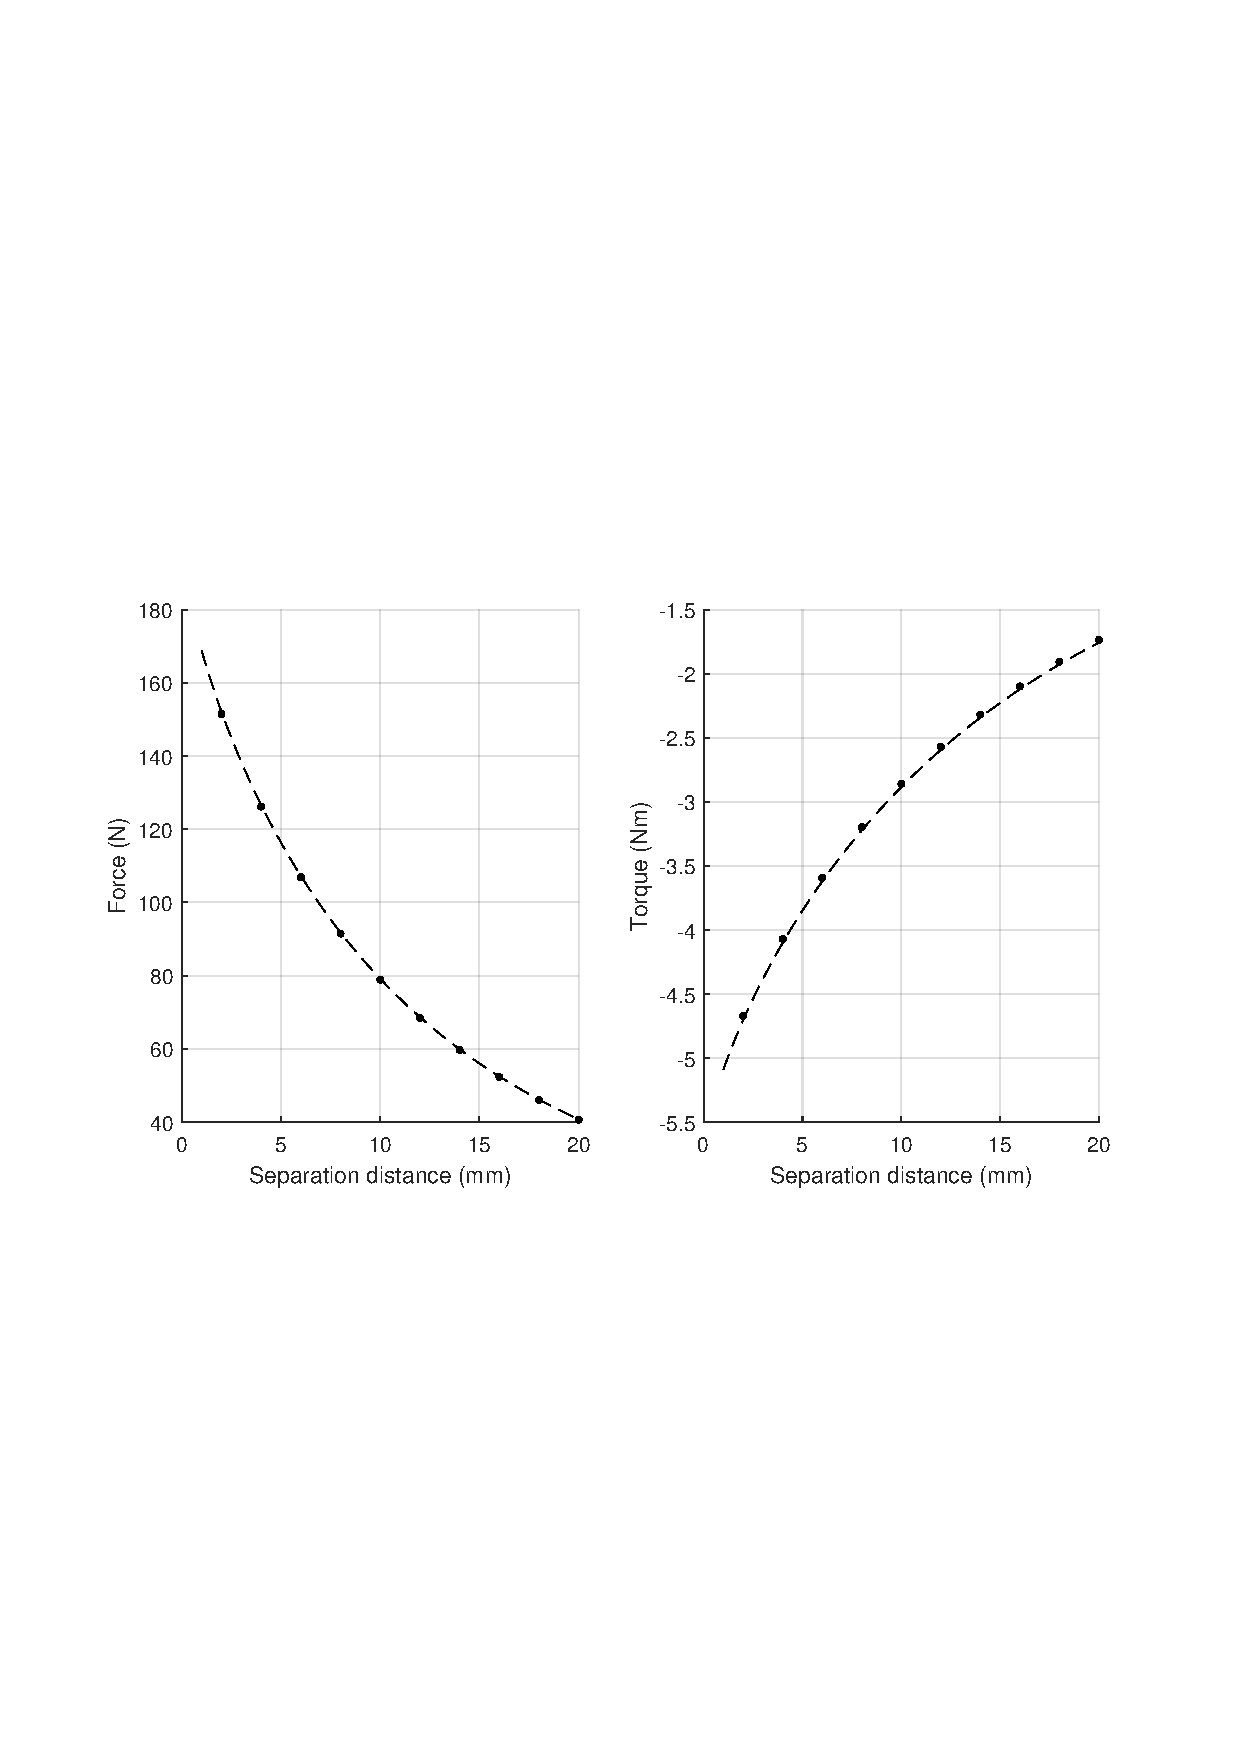
\includegraphics[trim = 3cm 9cm 3cm 9cm,width=0.9\linewidth]{p1/p1FIG6}
	\caption{The \(x\)-force and \(y\)-torque on magnet B shown in Figure \ref{fig:p1dodecahedra}. Both magnets are regular dodecahedra with edge lengths of 20mm. The torque is evaluated about the centre of magnet B. Dashed lines represent the force and torque evaluated using Algorithms \ref{alg:p1alg1} and \ref{alg:p1alg2}, and dots represent the results from finite element simulations. The results from both methods are in agreement, indicating correct results from Algorithms \ref{alg:p1alg1} and \ref{alg:p1alg2}.}
	\label{fig:p1dodecahedraresults}
\end{figure*}

The results obtained from Algorithms \ref{alg:p1alg1} and \ref{alg:p1alg2} align well with the finite element simulations. This indicates that the algorithms produce accurate force and torque results for non-cuboidal polyhedral magnets with non-parallel magnetisation vectors, further validating Algorithms \ref{alg:p1alg1} and \ref{alg:p1alg2}.

No analytic solutions for dodecahedral permanent magnets exist, so the error of Algorithms \ref{alg:p1alg1}, \ref{alg:p1alg2}, and the finite element simulations cannot be quantified. However, the solution time can still be analysed. Algorithms \ref{alg:p1alg1} and \ref{alg:p1alg2} were again considerably faster than the finite element simulations, with solutions being completed in approximately 4.96 seconds using 4608 triangular elements on the surface of magnet B, while each finite element simulation took approximately 40-50 seconds using an adaptive setup with a percent error of 1\% and approximately 18000 tetrahedral elements.